% !TeX root = ../main.tex
% !TeX spellcheck = en_US

\chapter{Case Study: Binomial Heaps}
As an example of how to use the framework we developed in the last chapter, let us take a look at binomial heaps. A heap is a data structure designed for quick access (and usually removal) of a minimum element. Use cases include, among other things, priority queues and sorting algorithms.

\section{Theoretical Background}
First, we need to define binomial \emph{trees}. Binomial trees are already heaps in their own right, but with one notable restriction: The size of each trees is always a power of two. The logarithm of the size of a tree is called its rank.

A rank zero tree is just a single node:

\begin{figure}[h]
\begin{center}
    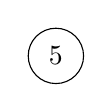
\begin{tikzpicture}

\node [shape = circle, minimum size = 2em, draw=black] at (0,0) {$5$};
\end{tikzpicture}
\end{center}
\end{figure}

A rank $n$ tree is a root node with $n$ children: the first a rank $n-1$ tree, the second a rank $n-2$ child and so on. The value of each child node must be larger than that of the root node.

\begin{figure}[h]
\begin{center}
    \begin{tikzpicture}

\node [shape=circle, minimum size = 2em, draw=black] (v1) at (0,0) {$3$};
\node [shape=circle, minimum size = 2em, draw=black] (v2) at (0,-1.5) {$6$};
\draw  (v1) edge (v2);
\node at (0,1) {Rank 1};
\node at (4.5,1) {Rank 2};
\node [shape=circle, minimum size = 2em, draw=black] (v3) at (4.5,0) {$2$};
\node [shape=circle, minimum size = 2em, draw=black] (v6) at (4.5,-1.5) {$5$};
\node [shape=circle, minimum size = 2em, draw=black] (v4) at (3,-1.5) {$4$};
\node [shape=circle, minimum size = 2em, draw=black] (v5) at (3,-3) {$7$};
\draw  (v3) edge (v4);
\draw  (v4) edge (v5);
\draw  (v3) edge (v6);
\node [shape=circle, minimum size = 2em, draw=black] (v7) at (11.5,0) {$3$};
\node [shape=circle, minimum size = 2em, draw=black] (v8) at (11.5,-1.5) {$9$};
\node [shape=circle, minimum size = 2em, draw=black] (v9) at (10,-1.5) {$6$};
\node [shape=circle, minimum size = 2em, draw=black] (v11) at (8.5,-1.5) {$7$};
\node [shape=circle, minimum size = 2em, draw=black] (v10) at (10,-3) {$7$};
\node [shape=circle, minimum size = 2em, draw=black] (v12) at (8.5,-3) {$9$};
\node [shape=circle, minimum size = 2em, draw=black] (v13) at (7,-3) {$9$};
\node [shape=circle, minimum size = 2em, draw=black] (v14) at (7,-4.5) {$9$};
\draw  (v7) edge (v8);
\draw  (v7) edge (v9);
\draw  (v9) edge (v10);
\draw  (v7) edge (v11);
\draw  (v11) edge (v12);
\draw  (v11) edge (v13);
\draw  (v13) edge (v14);
\node at (11.5,1) {Rank 3};
\end{tikzpicture}
\end{center}
\caption{Binomial trees of higher ranks}
\label{fig:binomial:rankn}
\end{figure}

We can join (or link) two trees of the same rank quickly by comparing their root nodes. The tree with the larger root becomes a child of the tree with the smaller one, increasing the rank of the new tree by one (\autoref{fig:binomial:merge}).

\begin{figure}[h]
\begin{center}
    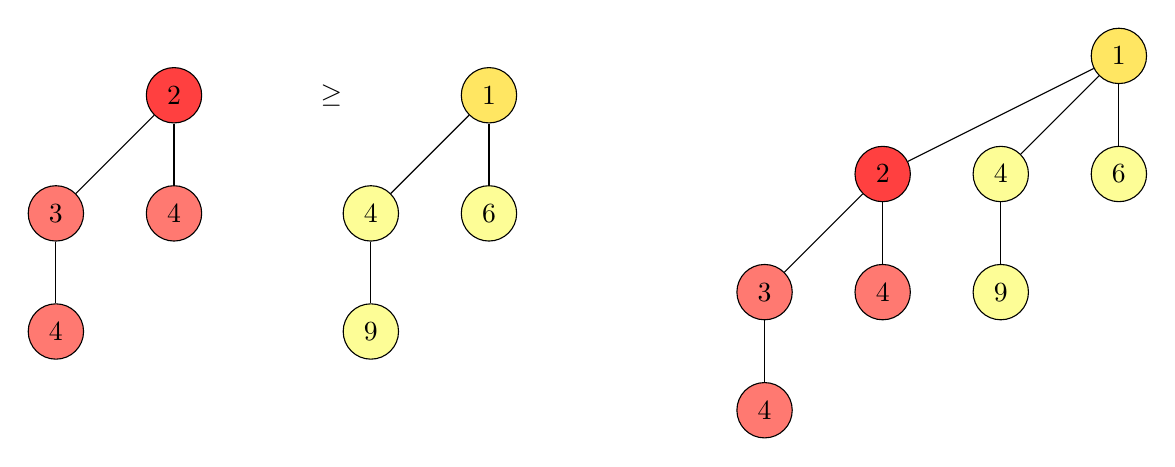
\begin{tikzpicture}
\definecolor{pastel-red}{HTML}{FF7971}
\definecolor{pastel-yellow}{HTML}{FDFD96}
\definecolor{sat-yellow}{HTML}{FFE662}
\definecolor{sat-red}{HTML}{FF4040}

\node [shape = circle, minimum size = 2em, draw = black, fill = sat-red] (v1) at (0,0) {$2$};
\node [shape = circle, minimum size = 2em, draw = black, fill = pastel-red] (v2) at (0,-1.5) {$4$};
\node [shape = circle, minimum size = 2em, draw = black, fill = pastel-red] (v3) at (-1.5,-1.5) {$3$};
\node [shape = circle, minimum size = 2em, draw = black, fill = pastel-red] (v4) at (-1.5,-3) {$4$};
\node [shape = circle, minimum size = 2em, draw = black, fill = sat-yellow] (v5) at (4,0) {$1$};
\node [shape = circle, minimum size = 2em, draw = black, fill = pastel-yellow] (v6) at (4,-1.5) {$6$};
\node [shape = circle, minimum size = 2em, draw = black, fill = pastel-yellow] (v7) at (2.5,-1.5) {$4$};
\node [shape = circle, minimum size = 2em, draw = black, fill = pastel-yellow] (v8) at (2.5,-3) {$9$};
\draw  (v1) edge (v2);
\draw  (v1) edge (v3);
\draw  (v3) edge (v4);
\draw  (v5) edge (v6);
\draw  (v5) edge (v7);
\draw  (v7) edge (v8);
\node at (2,0) {$\geq$};
\node at (6,-1.5) {$\implies$};


\node [shape = circle, minimum size = 2em, draw = black, fill = sat-red] (v21) at (9,-1) {$2$};
\node [shape = circle, minimum size = 2em, draw = black, fill = pastel-red] (v22) at (9,-2.5) {$4$};
\node [shape = circle, minimum size = 2em, draw = black, fill = pastel-red] (v23) at (7.5,-2.5) {$3$};
\node [shape = circle, minimum size = 2em, draw = black, fill = pastel-red] (v24) at (7.5,-4) {$4$};
\node [shape = circle, minimum size = 2em, draw = black, fill = sat-yellow] (v25) at (12,0.5) {$1$};
\node [shape = circle, minimum size = 2em, draw = black, fill = pastel-yellow] (v26) at (12,-1) {$6$};
\node [shape = circle, minimum size = 2em, draw = black, fill = pastel-yellow] (v27) at (10.5,-1) {$4$};
\node [shape = circle, minimum size = 2em, draw = black, fill = pastel-yellow] (v28) at (10.5,-2.5) {$9$};
\draw  (v25) edge (v26);
\draw  (v25) edge (v27);
\draw  (v27) edge (v28);
\draw  (v25) edge (v21);
\draw  (v21) edge (v22);
\draw  (v21) edge (v23);
\draw  (v24) edge (v23);
\end{tikzpicture}
\end{center}
\caption{Merging two binomial trees}
\label{fig:binomial:merge}
\end{figure}

Using these trees, we can now construct a binomial heap capable of storing any number of elements. We model a heap as a list of binomial trees of strictly increasing rank. A heap with $n$ elements has at most $1 + \lfloor \log_2 n \rfloor$ elements: The largest tree in this heap has rank $\lfloor \log_2 n \rfloor$ and then there can be only $\lfloor \log_2 n \rfloor$ trees with a smaller rank.

To find the minimum element, we iterate over all trees in the heap, finding the minimum among their root elements. Since there are only $\log n$ trees, this runs in $\mathcal O(\log n)$